\documentclass[conference]{IEEEtran}
\usepackage{amssymb}
\usepackage{amsmath}
\usepackage{graphicx}
\usepackage[draft]{hyperref}
\hyphenation{op-tical net-works semi-conduc-tor}

\begin{document}

\renewcommand{\figureautorefname}{Fig.}
\newcommand{\subfigureautorefname}{Fig.}
\renewcommand{\sectionautorefname}{Section}
\renewcommand{\subsectionautorefname}{Section}

\title{EEL6935 Course Project Midterm Report \\
    Sentiment Analysis}
\author{\IEEEauthorblockN{
    Caleb Bryant\IEEEauthorrefmark{1},
    Jixin Feng\IEEEauthorrefmark{2}}
\IEEEauthorblockA{Department of \\
    \IEEEauthorrefmark{1} Computer \& Information Science \& Engineering\\
    \IEEEauthorrefmark{2} Electrical \& Computer Engineering\\
    University of Florida,
    Gainesville, FL, 32611\\
    Email: \texttt{{\small\{cal2u,fengjixin\}}@ufl.edu}}}

\maketitle

\begin{abstract}
    The volume of text on the Internet -- unstructured text especially --
    is increasing with drastic speed everyday. Unlike
    human brains, traditional computer programs lack the ability of extracting
    useful information from unstructured text with satisfactory precision.
    While traditional machine learning programs have had limited success
    on NLP problems based on ``bag of words'' models and feature engineering,
    deep learning and the development of word embeddings have shown
    promising results without the need for feature engineering. For this course
    project for EEL6935 Big Data Ecosystems, we propose to implement a sentence 
    classification program based on convolutional neural networks (CNN) and 
    compare the performance with a logistic regression based baseline model.
    
\end{abstract}

\IEEEpeerreviewmaketitle

\section{Introduction}
\label{intro}
    With the tremendous volume of unstructured text generated everyday, on or off
    internet, the demands for processing and extracting useful information
    from it has been constantly increasing. It is predicted that by 2020 the
    total data volume of ``digital universe'' will increase to 40 ZB
    ($40\times 10^{21}$ bytes), which is about 50 times more than the size of
    year 2010\cite{gantz2012digital}. Most of the text will be generated by various
    sources like news media, social networks, medical records, etc.

    Although this text data is a valuable source of information
    and can be easily comprehended by humans, current computational methods
    continue to struggle extracting information from unstructured text 
    sources.
    Hence effective methods to process and analyze unstructured text data are
    desperately needed.

    In this course project, we are targeting a specific domain of text analysis
    problems -- sentiment analysis. The goal of sentiment analysis is to assign
    proper pre-defined sentiment labels to a given text, so that the emotion behind the
    sentence can be represented and then categorized\cite{allahyari2017brief}.
    Mathematically, the classification model can be represented as:
    $$f:\mathcal{D}\rightarrow\mathcal{L}$$
    where $\mathcal{D}=\{d_0, d_1,\ldots, d_{n-1}\}$ is the set of sentences
    , and $\mathcal{L}=\{l_0, l_1,\ldots, l_{k-1}\}$ is the set of labels.
    Depending on whether multiple labels are allowed to assigned to a document, the
    classification is called soft or hard\cite{gopal2010multilabel}. In the sentiment 
    analysis scenario, the set of labels is usually binary, this can be used
    to model the overall opinion the subject received. Movie review, for example,
    can be labeled as like/dislike, positive/negative, happy/sad, etc.
    \cite{pang2002thumbs}

    The performance of a sentiment analysis system can be evaluated with its
    F-1 score, which can be defined as\cite{forman2003extensive}:
    $$F_1=\frac{2}{\frac{1}{r}+\frac{1}{p}}=\frac{2pr}{p+r}$$
    where $p=\frac{tpr}{tpr+fpr}$ stands for precision and $r=\frac{tpr}{tpr+fnr}$
    stands for recall.

    Historically, sentiment analysis has been done via statistical
    and machine learning methods like Naive Bayes, k-nearest neighbors, decision
    trees, SVM, etc. In this report, we decide to compare the performance of
    sentence classifier based on different techniques: 
    classic Bag-of-Words\cite{pang2002thumbs},
    Convolutional Neural Network (CNN)\cite{kim2014convolutional} 
    and Long Short-Term Memory (LSTM)\cite{barnes2017assessing}.
    
    Due to the strict limit of time and man-power, our whole vision of this course 
    project may not be fulfilled in time. Hence, we carefully divided our goals into 
    two sets: project core and stretched goals. The sentiment analysis via 
    Logistic Regression and CNN are the core of our project hence we aim to 
    finish them by the end of semester, the analysis based on LSTM and more
    user-friendly interface of the simulation program, on the other hand,
    may end up with uncertain progress, but we will still try to finish them 
    with our best effort.
    
    The report is organized as follows: 
    A brief introduction of related research contribution is in \autoref{related}.
    system architecture and different analysis approaches are introduced and compared 
    in \autoref{model}.
    The benchmarks used for evaluating the performance is explained in 
    \autoref{performance}
    simulation scenarios are listed in \autoref{scenarios}.
    The current progress and future plan of the whole project, and team management
    is reported in \autoref{manage}
    
\section{Related Work}
\label{related}
    When processing natural languages, conventional methods usually treat text as 
    a stream of bytes or words, and don't put much consideration into the relations
    between them. This create simplicity but failed at digging the meaning of
    language. Vectorize words in texts has been proof successful for numerous NLP
    tasks. Researchers in Google spend a lot of efforts on this topic and 
    made quite noticeable contributions\cite{mikolov2013efficient, word2vec}.
    
    Sentiment analysis has been actively studied for a long time. At the very beginning
    of research, the analysis usually focused on analyze the sentiment of entire
    sentense/document\cite{sack1994computation}. The application of
    text vectorization and conventional machine learning techniques had great
    success in 2000s\cite{pang2002thumbs}. With the help of significantly improved
    computation power of CPU and GPU, the neural network related techniques 
    started to show great potential in sentiment analysis 
    domain\cite{kim2014convolutional,barnes2017assessing}.
    
\section{System Architecture}
\label{model}
\subsection{Project Core}
\label{model:core}
    In this course project, we want to implement a convolutional neural network
    model for text sentiment analysis, and compare its performance to a baseline
    generated by the bag-of-words model paired with conventional machine learning
    techniques, logistic regression.
    
\subsubsection{Bag-of-Words}
\label{model:core:bow}
    Traditionally, sentiment analysis can be done by conventional machine learning
    methods like Na\"ive Bayes, maximum entropy, logistic regression and 
    support vector machine (SVM). 
    
    Computer programs can only treat text as an array of characters, 
    in order to feed text to machine learning models in this project, we need to 
    convert conventional text into mathematically representable forms. In this
    paper, we use vector space model to represent the sentences to be analyzed.
    Depending on the research domain, this can be called Bag-of-Words model, 
    Bag-of-Features model or Vector Space model\cite{salton1975vector}.
    
    Let $$\mathcal{W}=\{w_0, w_1,\ldots, w_{m-1}\}$$ be a m-word predefined set. Each 
    word in $\mathcal{W}$ is a word chosen to be a feature appears in sentence and 
    considered by our machine learning model.
    
    Let $n_j(d_i)$ be the metric of word $w_j$ appears in sentence $d_i$, hence each 
    sentence can be converted into vector representation 
    $$\bar{d_i}=(n_0(d_i),n_1(d_i),\ldots,n_{m-1}(d_i))$$.
    
    Depending on how metrics of words are defined, the vector representation can be
    generally categorized into feature frequency representation and feature presence
    representation\cite{pang2002thumbs}.


\subsubsection{Convolutional Neural Network}
\label{model:core:cnn}
    CNN uses multiple layers of convolving filters that apply on the input data and
    calculate the output after all feeding the input through all of the layers. Although
    originally built for computer vision, CNNs have shown quite significant potential in
    natural language processing (NLP), and especially in sentence classification.
    Our chosen network architecture is based upon Yoon Kim's work on sentence
    classification\cite{kim2014convolutional}. The architecture consists of four 
    main parts: a word
    embedding layer, a convolution layer, a pooling layer and a fully connected layer
    at the end.
    \begin{figure*}
    \center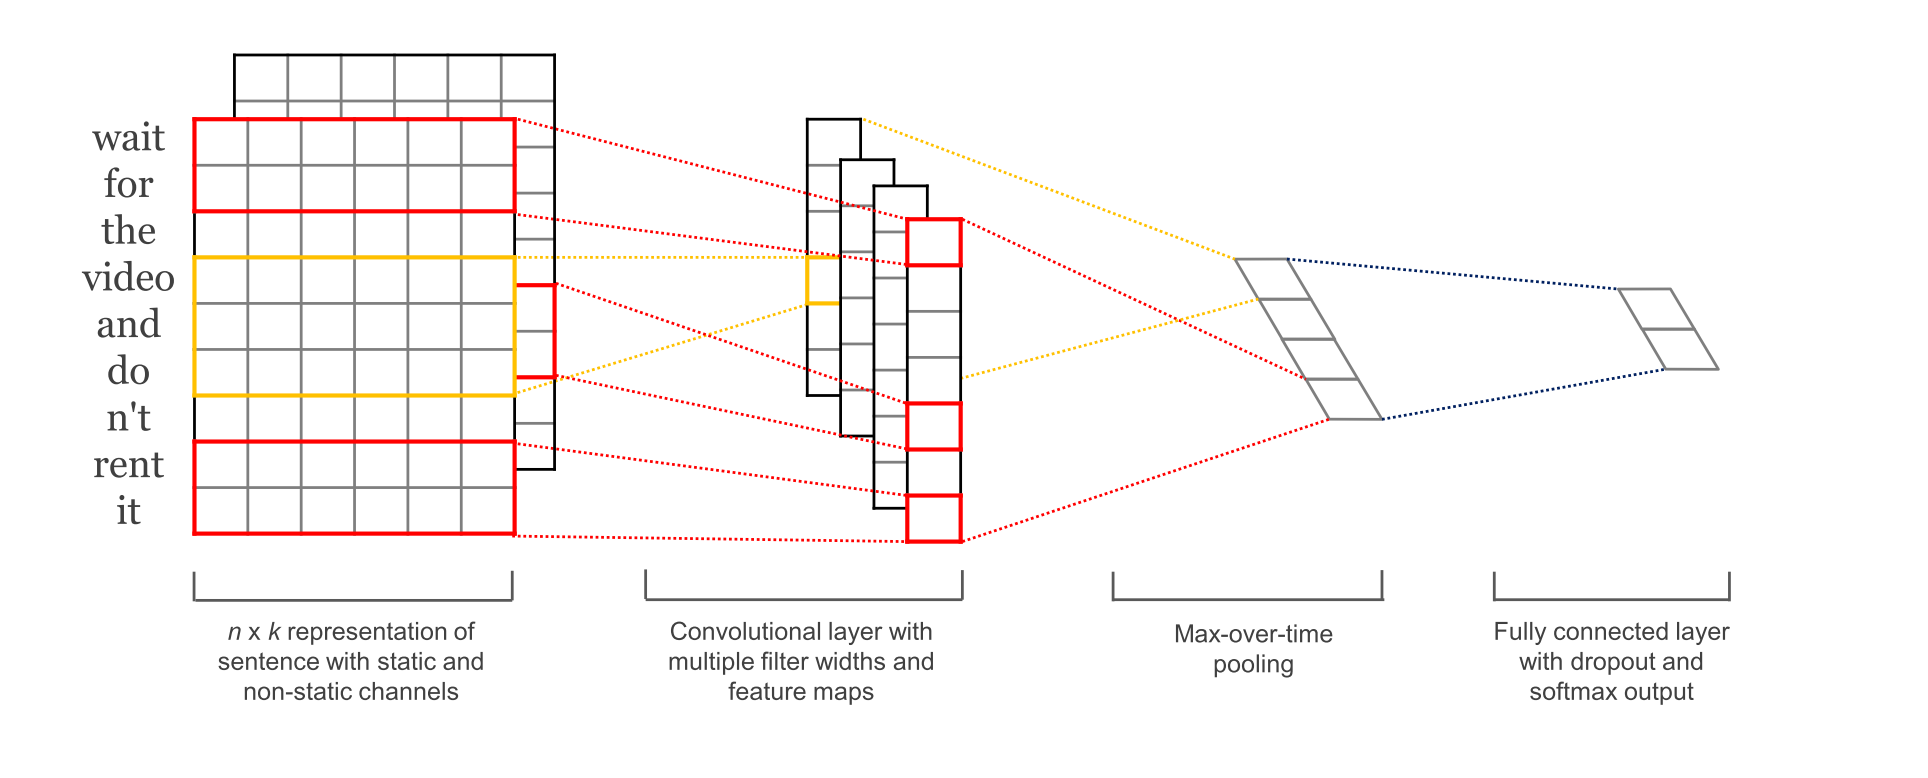
\includegraphics[width=0.9\textwidth]{figure/sc_model}
    \caption{Model architecture with two channels for an example sentence,
     figure credit: \cite{kim2014convolutional}}
    \end{figure*}

    Distributed word embeddings, proposed by Mikolov et al.
    in 2013\cite{word2vec}, allow us to represent a word as a vector in
    multi-dimensional space, and they form the basis for feeding text into our deep
    learning model.

    Let $x_{i} \in \mathbb{R}^k$ be a dimentional word vector representing the $i$-th word in the
    sentence. Thus, the sentence would be represented by
    \begin{equation}
    x_{1:n} = x_1 \oplus x_2 \oplus ... \oplus x_n
    \end{equation}
    Where $\oplus$ signifies concatenation. Suppose $x_{i:i+j}$ refers to concatenating
    word vectors $x_i, x_{i+1}, ... , x_{i+j}$. The convolution operator with a filter
    $W \in \mathbb{R}^{hk}$ applied to a window size of $h$
    words is defined as
    \begin{equation}
    c_i = f(W \cdot x_{i:i_{h-1}} + b)
    \end{equation}
    Where $b$ is a bias term and $f$ signifies a non linear function such as the hyperbolic
    tangent. We use this filter to generate a feature map $c = [c_1, c_2, ... ,x_{n-h+1}]$
    with $c \in \mathbb{R}^{n-h+1}$ by applying the filter to each possible window of words in
    the sentence $x_{1:h}, x_{2:h+1}, ... ,x_{n-h+1:n}$.

    We plan to use multiple filters with varying window sizes to obtain multiple features, and we will
    compare our results for different hyperparameters.
    A max-over-time pooling operation $\hat{c}$ = max\{$c$\} will be applied once the feature
    maps are generated. The pooling operation outputs the largest value from each individual
    feature maps. We will employ dropout on the penultimate layer $z = [\hat{c}_1,...,\hat{c}_m]$
    (we have $m$ filters) for regularization with a constraint on $l_2$-norms of the weight
    vectors. This should help prevent co-adaptation of hidden units by randomly setting weights
    to zero for selected neurons. The function is expressed below:

    \begin{equation}
    y = W \cdot (z \circ r) + b
    \end{equation}

    where $\circ$ is the element-wise multiplication operator and $r \in \mathbb{R}^m$ is
    the masking vector of Bernoulli random variables with probability $p$ of being 1.
    The gradients are backpropagated through the unmasked units during training. At test
    time, the learned weight vectors are scaled by $p$ such that $\hat{w} = pw$ and $\hat{w}$
    is used to score unseen sentences. Finally, we will constrain $l_2$-norms of the weight
    vectors by rescaling $w$ to have $||w||_2 = s$ whenever $||w||_2 > s$ after a gradient
    decent step.

\subsection{Stretched Goals}
\label{model:stretch}
    
    Beside this, we also plan to build a web-based interface for the simulation, aiming
    to increase the user-friendliness of the whole project. The detail of the stretched
    goal is still yet to be fixed, and it will be will be included in the final project
    report once finished. 

\subsubsection{Long Short-Term Memory (LSTM)}
\label{model:stretch:lstm}
    LSTM was originally proposed by Sepp Hochreiter and J\"urgen Schmidhuber back in 
    1997\cite{hochreiter1997long}, and usually serves as a building block of larger
    recurrent neural network (RNN) layers. The basic object of LSTM is to fine-tune
    the memory length of the input and system state over an arbitrary period of time
    hence preventing premature ``memory loss'' and gradient vanishing of RNN.
    
    Given a word sequence $S=\{w_0,w_1,\ldots,w_{l-1}\}$ with length $l$, the states
    of LSTM are updated as:
    $$
    \begin{bmatrix} 
    i_t\\f_t\\o_t\\c_t 
    \end{bmatrix} = 
    \begin{bmatrix}
    \sigma\\\sigma\\\sigma\\\tanh
    \end{bmatrix}
    S[h_{t-1},x_t]
    $$
    , in which $c_t=f_t\circ c_{t-1} + i_t\circ\hat{c_t}$ and $h_t=o_t\circ\tanh{c_t}$.
    At time $t$ in this relationship, $c_t$ and $h_t$ are the LSTM memory and 
    hidden state, $\hat{c_t}$ is the current cell state. The input at time $t$ 
    is $x_t$ and the input/forget/output gate activation are represented by $i$, 
    $f$ and $o$ respectively. $\sigma$ and $\circ$ are notations of logistic 
    sigmoid function and element-wise multiplication\cite{zhou2016text}.
    
    Depending on the requirement on system causality, the LSTM can be applied on
    both directions of time, which becomes Bidirectional LSTM 
    (BLSTM)\cite{schuster1997bidirectional,barnes2017assessing}.

\subsubsection{Web Interface}
\label{model:stretch:web}
    To improve the user-friendliness of this project, we also plan to create a 
    web-based user interface for the program. With a webpage, selecting
    the model for sentiment analysis can be done in a mouse click instead of 
    enter a series of command line parameters, the output can also
    be read from web browser, not a standard output stream in terminal. 

\section{Performance Evaluation}
\label{performance}


\section{Proposed Simulation Scenarios}
\label{scenarios}
    To test and evaluate our model, we propose using the Stanford Large Movie Review
    Dataset to preform sentiment classification\cite{maas2011learning}.
    The dataset contains 50,000 highly polar
    movie reviews, and we will score each movie review as either positive or
    negative. We will use a 60/20/20 split for training, development, and testing.

    In addition to using the above data set, we will also train and test using the 
    Stanford Sentiment Treebank, which is one of the data sets Kim evaluated in 
    his paper\cite{sentimenttreebank}. Using the same data set
    will allow us to compare our model with Kim's model directly. 
    Both binary (positive/negative) and fine-grained (scale from 1-5) 
    classification tasks will be performed and scored for accuracy.
    For all tasks, we will compute the accuracy of our model by diving the 
    number of correct classifications by the total number of test samples.

    We will be implementing the model using Python 3 and Tensorflow
    \cite{tensorflow2015-whitepaper}. The 
    simulations will be conducted on computers with a 3.1GHz Intel Core i7 
    CPU with 8MB cache, 16GB RAM and nVidia GTX 1050 GPU with 4GB memory 
    running Ubuntu 14.04 LTS.

\section{Current Progress and Project Management}
\label{manage}

    In this proposal we presented a convolutional neural network based on 
    Kim's paper for sentiment analysis on a number of data sets. We have 
    also proposed a test plan to evaluate the performance of our deep 
    learning architecture.

\bibliographystyle{IEEEtran}
\bibliography{eel6935_mid_report.bib}

\end{document}
